\subsection{传输对象模式}

传输对象模式(Transfer Object Pattern)是一种用于从客户端向服务器一次性传递大量数据的轻量级模式。它通过将数据封装在一个对象中,并将这个对象用作客户端和服务器之间的数据传输方式,来简化客户端和服务器之间的通信。

传输对象模式常用于分布式系统中,它可以帮助减少系统中各个部分之间的通信复杂度,提高系统的性能。例如,一个分布式电商系统中,客户端可能需要检索大量的商品信息,如果每次检索都需要将所有信息一次性传送给客户端,这将会极大地降低系统的性能。使用传输对象模式,可以将所有商品信息封装在一个传输对象中,并由服务器端一次性传送给客户端,从而避免了频繁的网络通信,提高了系统的性能。

\begin{figure}[H]
  \centering
  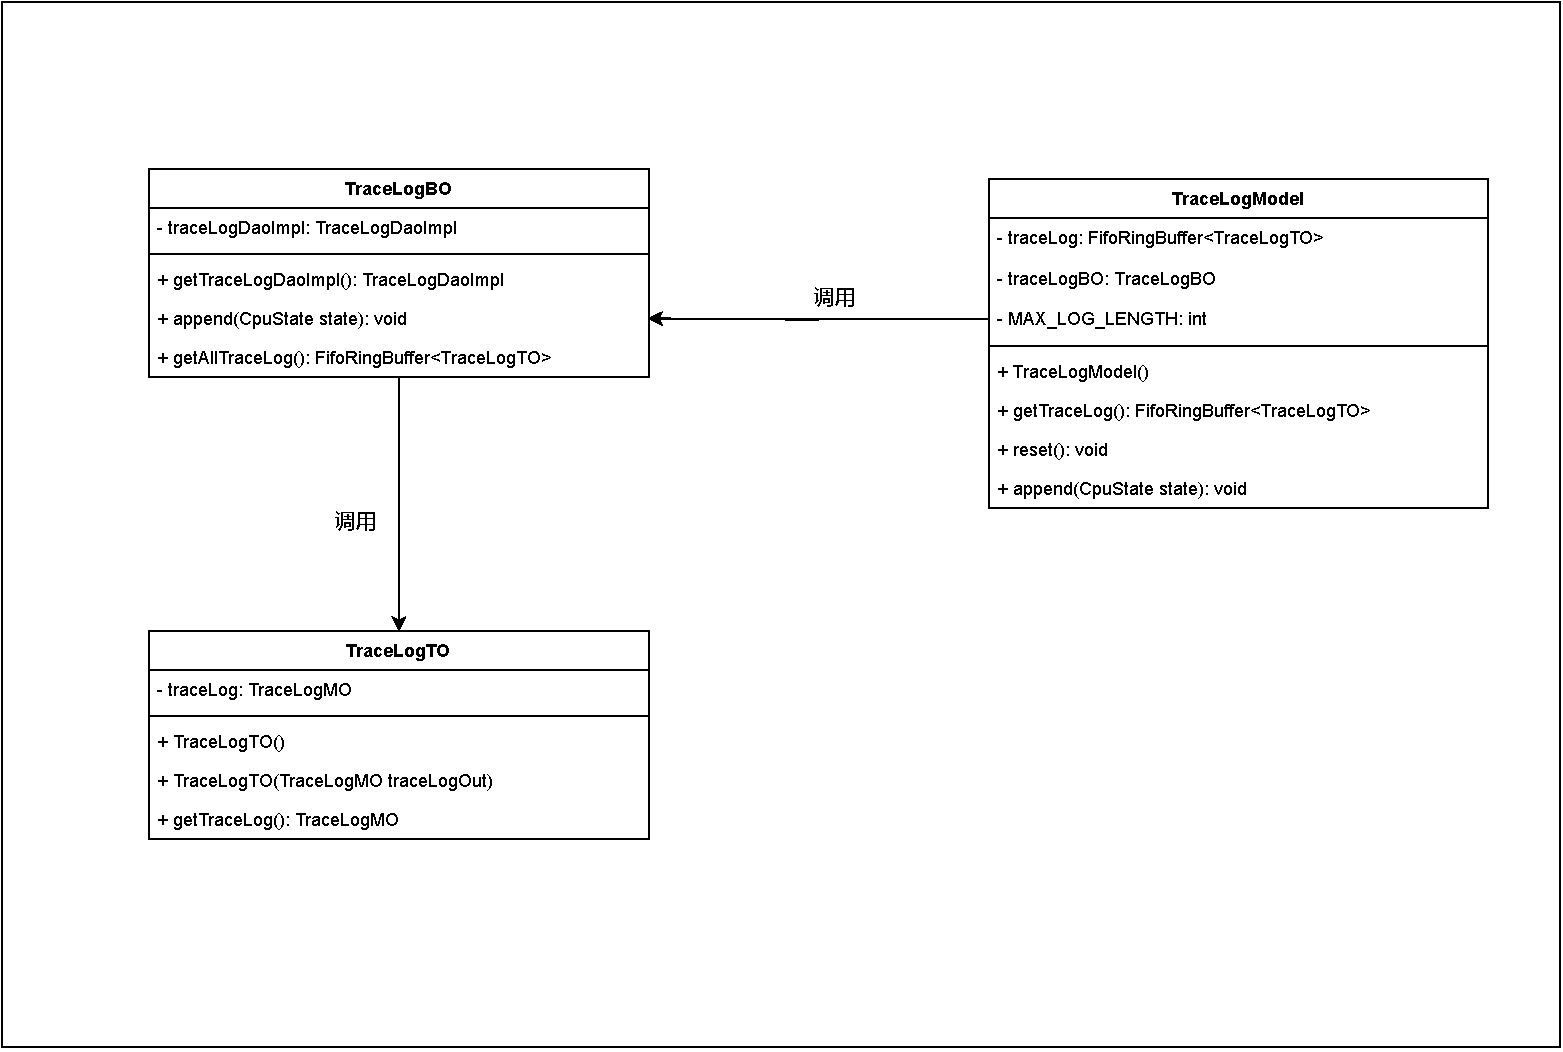
\includegraphics[width=0.9\textwidth]{figures/传输对象模式.pdf}
  \caption{传输对象模式在 Slow6502 中的类图}
\end{figure}

在这里我们设计了TraceLogTO类作为要传输的业务对象,其内部包含了TraceLogMO类的数据。设计TraceLogBO类作为业务对象类,用于向客户端(即MVP模式中的TraceLogModel类)传输数据,以及从客户端获取新添加的traceLog信息。

